

\section{Spiral Density Waves}

Introduce spiral arms and density waves in the context of observations. Mention Lin-Shu hypothesis and lead into tidal interaction which is what we care about here.

\subsection{Spiral Structure Preliminaries}
We now introduce the following concepts:
\begin{enumerate}
    \item The \textit{pitch angle} $\alpha$: a spiral arm is defined as the angle between the tangent to the spiral at some radius $r$ and the circle with the same radius. 
    Thus $\alpha$ is in general a function of radius and $0 < \alpha < \pi/2$ by definition.
    \item $m$-fold \textit{rotational symmetry}: if a rotation of $2\pi/m$ radians results in no change to the disk surface density, that is $\Sigma(r,\phi)=\Sigma(r,\phi+\frac{2\pi}{m})$, then the disk is said to contain $m$ spiral arms and exhibits an $m$-fold rotational symmetry. 
    For example, a disk containing two spiral arms will be unchanged under a rotation of $180^\circ$ and so has $2$-fold rotational symmetry.
    \item \textit{Leading} and \textit{trailing} spiral arms: the tip of a leading spiral arm points in the direction of the bulk rotation of the disk, while the tip of a trailing arm points in the opposite direction to the rotation. 
    While it seems that leading arms may indeed be physically realised in the universe \citep[eg.][]{vaisanen2008}, they are at minimum very rare. 
    We will be concerned only with trailing spirals in this thesis.
%    \item The \textit{pattern speed} $\Omega_\mathrm{p}$: In the Lin-Shu hypothesis the spiral structure is a fixed pattern that rotates rigidly. 
%    The angular speed of rotation of these spirals according to some inertial observer is known as the pattern speed $\Omega_\mathrm{p}$. 
%    More generally, the pattern speed is well defined so long as the spirals constitute a steady state solution in some rigidly rotating frame. 
%    As we will see, this is the case for the spiral wake generated by a perturbing planet on a circular orbit, in which case the pattern speed is simply equal to the orbital rotation of the planet
\end{enumerate}

Consider a disk containing a set of $m$ spiral arms such that is has $m$-fold symmetry. We may parameterise the curves defined by the centre of each of the spiral arms as
\begin{align}
    m\phi + f(r,t) = C \,\, \mathrm{mod} \,\, 2\pi, \label{eq:spiral_para}
\end{align}
where $C$ is a constant real number and $f$ is known as the \textit{shape function}. The \textit{radial wavenumber} $k$ is defined in terms of $f$ and is given by
\begin{align}
    k(r,t) \equiv \partial_r f(r,t).
\end{align}
For a counter-clockwise rotating disk we have $m>0$ and so $k>0$ corresponds to trailing arms while $k<0$ gives leading arms. 
The opposite is true for clockwise rotating disks with $m<0$. 
We will always assume both $k$ and $m$ are positive, corresponding to tailing arms in a counter-clockwise rotating disk. 
The pitch angle of a spiral arm is given by
\begin{align}
    \mathrm{cot}\,\alpha = \left| r \partial_r \phi \right|,
\end{align}
where $r \partial_r \phi$ is evaluated along the curve that defines the spiral. In terms of the parameterisation \ref{eq:spiral_para} we have $\partial_r[m\phi+f(r,t)] = m \partial_r \phi + k = 0$ giving
\begin{align}
    \alpha = \arctan \left( \frac{m}{kr} \right). \label{eq:pitchangle}
\end{align}

\subsection{No Leading Spirals}

In the previous section we stated that while leading spirals may exist in nature, they are at least much rarer that than trailing spirals. 
Indeed, there are \textbf{no} known examples of leading spirals in circumstellar disks.
This state of affairs is at least initially puzzling; if the trailing spiral arms seen in astrophysical disks are steady state solutions governed by Newtonian physics, which is fully time-reversible, surely the corresponding leading spirals solution is entirely equivalent?
\citet{lynden-bell1967} followed this argument to prove the \textit{anti-spiral} theorem, which states that if trailing spirals constitute a steady state solution to time-reversible equations, then there necessarily exists an equivalent leading spiral solution.
Thus the apparent ubiquity of trailing spirals in nature tells us that either the governing physics is not time-reversible, or the spirals are not true steady state solutions.
In the latter case spiral structure may be the result of a recent disturbance, or may be continuously regenerated for example by period tidal forcing.
In the following section we will see that the perturbations driven by a gravitating body embedded in a circumstellar disk result in a trailing spiral structure that is a steady state solution.

\section{The Linear Disk Response}

\note{need a connecting sentence here to explain that we are eventually looking for the respone from a perturbing gravitating body.}

The 2D inviscid equations of momentum and continuity expressed in terms of surface density are given by 
\begin{align}
    &\partial_t u + u \partial_r u + \frac{v}{r} \partial_\phi u - \frac{v^2}{r} = - \partial_r \Phi - \frac{1}{\Sigma} \partial_r P, \label{eq:mom_eq_u} \\ 
    &\partial_t v + u \partial_r v + \frac{v}{r} \partial_\phi v - \frac{uv}{r} = - \frac{1}{r} \partial_\phi \Phi - \frac{1}{r\Sigma} \partial_\phi P, \label{eq:mom_eq_v} \\
    &\partial_t \Sigma + \frac{1}{r} \partial_r (r \Sigma u) + \frac{1}{r} \partial_\phi (\Sigma v) = 0. 
    \label{eq:cont_2d}
\end{align}
Assuming a polytropic equation of state
\begin{align}
    P = K \Sigma^\gamma,
\end{align}
where $K$ is a constant and $\gamma$ is the adiabatic index. We then find the sound speed $c$ to be
\begin{align}
    c^2 = \partial_\Sigma P = \gamma K \Sigma^{\gamma-1}. \label{eq:cs_poly}
\end{align}
To simplify the equations we introduce the specific enthalpy $h$. Since the equation of state we are using is isentropic, we have $dh = dP / \Sigma$ giving
\begin{align}
    h = \int \frac{1}{\Sigma} dP = \int \frac{c^2}{\Sigma} d\Sigma = \frac{\gamma}{\gamma-1} K \Sigma^{\gamma-1}. \label{eq:enthalpy}
\end{align}
Note that
\begin{align}
    \partial_x h = \frac{\gamma}{\gamma - 1} K \partial_\Sigma (\Sigma^{\gamma-1}) \partial_x \Sigma = \gamma K \Sigma^{\gamma-2} \partial_x \Sigma,
\end{align}
such that the right-hand sides of equations \ref{eq:mom_eq_u} and \ref{eq:mom_eq_v} become
\begin{align}
    - \partial_r \Phi - \frac{1}{\Sigma} \partial_r P = - \partial_r \Phi - \gamma K \Sigma^{\gamma-2} \partial_r \Sigma = - \partial_r (\Phi + h) \label{eq:mom_u_RHS},
\end{align}
and
\begin{align}
    - \frac{1}{r} \partial_\phi \Phi - \frac{1}{r\Sigma} \partial_\phi P = - \frac{1}{r} \partial_\phi (\Phi + h) \label{eq:mom_v_RHS},
\end{align}
respectively.

We now perform a linear perturbation study; we assume that the spiral waves in the disk constitute only a small perturbation from some background steady-state, and that the background state is axisymmetric.
We rewrite the quantities $\Sigma,\Phi,h,u,v$ as a combination of the background value (denoted by subscript 0) and a small perturbation  (denoted by $\delta$)
\begin{align}
    \Sigma &= \Sigma_0 + \delta\Sigma \label{eq:pertsig} \\
    \Phi &= \Phi_0 + \delta\Phi \label{eq:pertphi} \\
    h &= h_0 + \delta h \label{eq:perth} \\
    v &= v_0 + \delta v \label{eq:pertv} \\ 
    u &= \delta u, \label{eq:pertu}
\end{align}
where we note that $u_0=0$ since we assume no radial motion in the background state.
From equations \ref{eq:mom_eq_u} and \ref{eq:mom_u_RHS}, and making use of the axisymmetry of the background state, we find the equation of motion for the background
\begin{align}
    \frac{v_0^2}{r} = \partial_r \left( \Phi_0 + h_0  \right), \label{eq:pertback}
\end{align}
which is the 2D equivalent of equation \ref{eq:rotation}. 
Substituting \ref{eq:pertsig}-\ref{eq:pertu} into equations \ref{eq:mom_eq_u}, \ref{eq:mom_eq_v}, \ref{eq:mom_u_RHS}, \ref{eq:mom_v_RHS}, discarding second order terms, and subtracting equation \ref{eq:pertback} yields the linearised equations of motion 
\begin{align}
    \partial_t \delta u + \Omega \partial_\phi \delta u - 2 \Omega \delta v &= - \partial_r \left( \delta \Phi + \delta h  \right) \label{eq:mom_u_lin} \\
    \partial_t \delta v + \Omega \partial_\phi \delta v - 2 B \delta u &= - \frac{1}{r} \partial_\phi \left( \delta \Phi + \delta h  \right), \label{eq:mom_v_lin}
\end{align}
where we have also substituted $v_0=\Omega r$ and the second Oort constant $B = -r \partial_r \Omega / 2 -\Omega$, which is related to the epicyclic frequency as $\kappa^2 = -4 B \Omega$. 
The linearised equation of continuity is obtained similarly from \ref{eq:cont_2d}
\begin{align}
    \partial_t \delta \Sigma + \frac{1}{r} \partial_r \left( r \Sigma_0 \delta u  \right) + \frac{\Sigma_0}{r} \partial_\phi \delta v + \Omega \partial_\phi \delta \Sigma. \label{eq:cont_lin}
\end{align}
We assume that the equations of motion \ref{eq:mom_u_lin} and \ref{eq:mom_v_lin} are solved by a summation of plane waves, where each perturbed quantity $a \in \left\{ \Sigma, \Phi, h, v, u \right\}$ can be written as
\begin{align}
    \delta a = \sum_m \delta a_m = \sum_m a_m(r) \exp \left[ i (m\phi - \omega t) \right]; \quad m \in \mathbb{Z}^{0+}, \label{eq:pert_sum_form}
\end{align}
where each $m$ component of the perturbation has $m$-fold symmetry and $a_m(r)$ is in general a complex function.
The physical perturbation is obtained by taking the real component $\mathrm{Re}(\delta a)$.
Substituting the summands of \ref{eq:pert_sum_form} in place of the perturbations in our linearised equations yields
\begin{align}
    u_m (r) &= \frac{i}{\Delta_m} \left[ (\omega - m \Omega) \partial_r (\Phi_m + h_m) - \frac{2 m \Omega}{r} (\Phi_m + h_m) \right] \label{eq:lin_u_m} \\
    v_m (r) &= - \frac{1}{\Delta_m} \left[ 2B \partial_r (\Phi_m + h_m) + \frac{m(\omega - m \Omega)}{r} (\Phi_m + h_m) \right] \label{eq:lin_v_m} \\
    \Sigma_m (r) &= \frac{1}{r(\omega - m \Omega)} \left[ m \Sigma_0 v_m -i \partial_r (r u_m \Sigma_0) \right] \label{eq:lin_cont_m},
\end{align}
where
\begin{align}
    \Delta_m \equiv \kappa^2 - (\omega - m \Omega)^2. \label{eq:def_delta_m}
\end{align}
Finally, we must linearise the equation of state.
Taking equation \ref{eq:enthalpy} and expanding in $\delta \Sigma / \Sigma_0$
\begin{align}
    h_0 + \delta h = \frac{\gamma}{\gamma - 1} K \Sigma_0^{\gamma - 1}(1 + \frac{\delta\Sigma}{\Sigma_0})^{\gamma-1} = \frac{\gamma}{\gamma - 1} K \Sigma_0^{\gamma - 1} + \gamma K \Sigma_0^{\gamma-1} \frac{\delta\Sigma}{\Sigma_0} + \mathcal{O}(\left(\delta\Sigma / \Sigma_0\right)^2).
\end{align}
Now substituting equations \ref{eq:cs_poly} and \ref{eq:enthalpy}, and taking only one component of the perturbation, we find
\begin{align}
    h_m \simeq c_0^2 \frac{\Sigma_m}{\Sigma_0}, \label{eq:lin_EOS_m}
\end{align}
where $c_0$ is the unperturbed sound speed.

With equations \ref{eq:lin_u_m}, \ref{eq:lin_v_m}, \ref{eq:lin_cont_m} and \ref{eq:lin_EOS_m} we have four constraints on the five state variables $\Sigma_m, \Phi_m, h_m, v_m$ and $u_m$.
We therefore now have a system of equations describing the \textit{linear response} of the disk $\Sigma_m$ for the azimuthal wave mode $m$, to the potential component $\Phi_m$.
By summing over all modes, we can calculate the \textit{global} response of the disk to some imposed gravitational potential.
This however, cannot be done analytically.

\subsection{Tightly-Wound Density Waves}

We now apply \textit{WKB approximation}, which will allow to find \textit{local} analytic solutions.
For spiral density waves this is equivalent to assuming that the spirals are \textit{tightly-wound} and thus is also called the \textit{tight-winding approximation}.
For a spiral with shape function $f$ let $\lambda_r$ be the radial separation between adjacent arms for fixed $\phi$, such that
\begin{align}
    2\pi = \left| f(r+\lambda_r, t) - f(r,t) \right|.
\end{align}
If we assume that the spirals are indeed tightly-wound such that $\alpha\rightarrow 0$, then we have that $f(r+\lambda_r,t)=f(r,t) + \lambda_r \partial_r f |_{r,t}$. 
Recalling that $\partial_r f |_{r,t}$ is none other than the radial wavenumber $k$, we find
\begin{align}
    2 \pi &= \left| f(r,t) + \lambda_r \partial_r f |_{r,t} - f(r,t) \right| \\
    &= \lambda_r | k | \\
    \Rightarrow \lambda_r &= \frac{2 \pi}{|k|},
\end{align}
and so we find that the radial wavenumber $r$ has the usual relationship with the radial wavelength $\lambda_r$ for tightly-wound spiral arms. 
Substituting equation \ref{eq:pitchangle} gives
\begin{align}
    \frac{2 \pi}{|rk|} &=  \frac{\tan \alpha}{m},
\end{align}
and so an equivalent condition for the tight-winding approximation is that $|rk| \gg 2 \pi$. 
This equivalency however does not hold for very large $m$ since the right-hand side above can then approach zero regardless of $\alpha$, and is also invalid for $m = 0$ ie. purely radial perturbations.

\subsection{Perturbed Potential under WKB}

We can write the perturbed spiral surface density for some mode $m$ in a form similar to \ref{eq:pert_sum_form} where we instead separate the rapid variations in density moving from one arm to another, and the slower variation while moving along a particular arm
\begin{align}
    \delta \Sigma_m = \Sigma_m \exp \left[ i \left( m \phi + f(r,t)  \right)  \right]. \label{eq:sigma_WKB}
\end{align}
To determine the disk response we must determine the gravitational potential due to this perturbed surface density, which is done by solving Poisson's equation
\begin{align}
    \nabla^2 \delta \Phi_m = 4 \pi G \delta \Sigma_m \delta(z), \label{eq:poisson_pert}
\end{align}
where $\delta(z)$ is the Dirac delta since we are working in 2D. 
The solution under the WKB approximation is \fct
\begin{align}
    \delta \Phi_m &= - \frac{2 \pi G}{|k|} \Sigma_m \exp \left[ i \left( m \phi + f(r,t)  \right)  \right] \\
    \Rightarrow \Phi_m &= - \frac{2 \pi G}{|k|} \Sigma_m. \label{eq:phi_m_sigma_m}
\end{align}

\subsection{The Lin-Shu Dispersion Relation} \label{sec:linshu}

We now rewrite each coefficient $a_m(r)$ for each term $\delta a_m$ of some perturbed quantity $\delta a$ as
\begin{align}
    a_m(r) = A_m(r) \exp \left[ i f(r) \right] = A_m(r) \exp \left[ i \int^r k(r') \, dr' \right], \label{eq:WKB_form}
\end{align}
where, similarly to \ref{eq:sigma_WKB}, $F(r)$ is a slowly varying function of radius and the exponential encapsulates more rapid variations. 
The radial derivative of $a_m$ is then
\begin{align}
    \partial_r a_m(r) = \left( \partial_r A_m + ikA_m  \right) \exp \left[ i \int^r k(r') \, dr' \right].
\end{align}
As shown in appendix \ref{appendix:asymptotic_deriv}, the WKB approximation implies that we may neglect the first term giving
\begin{align}
    \partial_r a_m(r) = ikA_m \exp \left[ i \int^r k(r') \, dr' \right] + \mathcal{O}\left(\frac{1}{|kr|}\right) \approx ik a_m(r). \label{eq:app_radial_deriv}
\end{align}
Thus assuming the form \ref{eq:WKB_form} for the quantities in equations \ref{eq:lin_u_m} - \ref{eq:lin_cont_m} and applying the WKB approximation yields
\begin{align}
    u_m(r) &= - \frac{k(\omega-m\Omega)}{\Delta_m} (\Phi_m + h_m) \label{eq:u_m_disp} \\
    v_m(r) &= - \frac{2ikB}{\Delta_m} (\Phi_m + h_m) \label{eq:v_m_disp} \\
    \Sigma_m(r) &= \frac{k \Sigma_0}{\omega-m\Omega} u_m, \label{eq:sigma_m_disp}
\end{align}
where the error is for all cases $\mathcal{O}(1/|kr|)$, as we have approximated the radial derivatives by \ref{eq:app_radial_deriv} and dropped terms proportional to $1/r$ in favour of terms proportional to $k$.
Finally, we may combine equations \ref{eq:lin_EOS_m}, \ref{eq:phi_m_sigma_m}, \ref{eq:u_m_disp} and \ref{eq:sigma_m_disp} to find the dispersion relation for tightly-wound density waves in a rotating gas disk
\begin{align}
    \left( \omega - m \Omega  \right)^2 &= \kappa^2 - 2 \pi G |k| \Sigma_0 + c_0^2 k^2. \label{eq:lin_shu_disp}
\end{align}
This result is known as the \textit{Lin-Shu Dispersion Relation} \citep{lin1964}.

\subsection{Stability}

If the right-hand side of the Lin-Shu dispersion relation \ref{eq:lin_shu_disp} is negative, that is $(\omega - m \Omega)^2 < 0$, then $\omega$ will become imaginary resulting in the exponential growth of the density perturbation $\delta \Sigma$.
By requiring that $(\omega - m \Omega)^2 > 0$ for all possible $k$, the disk stability criterion $Q$ is derived \citep{toomre1964}
\begin{align}
    Q(r) \equiv \frac{c_0 \kappa}{\pi G \Sigma} > 1.
\end{align}
Disk regions where $Q(r) < 1$ are subject to local unstable growth for certain values of $k$.
This may result in the fragmentation of the disk, and may be a pathway to the formation of giant planets \fct.
Planet formation through this mechanism is known as the Gravitational Instability model \fct, and it is similar in spirit to star formation through the Jeans instability \citep{jeans1902}.

\section{Planet Forcing}

\note{add connection paragraph maybe}

\subsection{Lindblad Resonances}

Let $(r,\phi)$ be polar coordinates centred on some star with mass $M_{\rm p}$.
We place a planet of mass $M_{\rm p} \ll M_\star$ on a circular orbit with radius $r_{\rm p}$ around the star.
The angular velocity of the planet $\Omega_{\rm p}$ will be given by 
\begin{align}
    \Omega_{\rm p}^2 = \Omega_{\rm K}(r_{\rm p}) = \frac{G M_\star}{r_{\rm p}^3} = \frac{1}{r_{\rm p}} \left( \frac{d\Phi_\star}{dr} \right) _{r_{\rm p}},
\end{align}
where $\Phi_\star$ is the gravitational potential for a point mass
\begin{align}
    \Phi_\star = - \frac{G m_\star}{r}.
\end{align}
Similarly, the angular velocity of some other test particle on a circular orbit (neglecting the influence of the planet) will be
\begin{align}
    \Omega_0^2 = \frac{1}{r} \frac{d\Phi_\star}{dr}.
\end{align}
Now consider the problem in a rotating frame such that the planet is always at $\phi=0$, which will remove the time dependence from the planet potential. 
The corresponding transformation will be given by $\phi \rightarrow \phi - \Omega_{\rm p} t$.
The Lagrangian for a test particle in such a frame is given by 
\begin{align}
    \mathcal{L} = \frac{1}{2} \left[ \dot{r}^2 + r^2 \left( \dot{\phi} + \Omega_{\rm p}  \right)^2 \right] - \Phi (r, \phi),
\end{align}
where $\Phi (r,\phi) = \Phi_\star (r) + \Phi_{\rm p} (r, \phi)$ is the total potential from both the star and planet.
From the Euler-Lagrange equations we find the equations of motion to be
\begin{align}
    \ddot{r} &= r \left( \dot{\phi} + \Omega_{\rm p} \right)^2 - \partial_r \Phi \label{eq:EOM_rad} \\
    r^2 \ddot{\phi} &= - 2 r \dot{r} \left( \dot{\phi} + \Omega_{\rm p}  \right) - \partial_\phi \Phi. \label{eq:EOM_az}
\end{align}
We now perform a perturbation study using the change of variables $r(t) \rightarrow r + \delta r (t)$  and $\phi (t) \rightarrow \phi (t) + \delta \phi (t)$ where we assume that $\delta r \ll r$ and $\delta \phi \ll \phi$.
We will similarly assume that $\Phi_{\rm p} \ll \Phi_\star$.
Thus the derivatives transform to first order as
\begin{align}
    \partial_r &\rightarrow \partial_r + \delta r \partial_r^2 r \\
    \partial_\phi &\rightarrow \partial_\phi + \delta \phi \partial_r^2 \phi.
\end{align}
The zeroth order terms of \ref{eq:EOM_rad} and \ref{eq:EOM_az} give 
\begin{align}
    r \left( \dot{\phi} + \Omega_{\rm p}  \right)^2 &= \frac{d\Phi_\star}{dr} , \\
    \ddot{\phi} &= 0
\end{align}
which is just the usual equations for centripetal acceleration. 
They are solved simply by associating $\dot{\phi}$ appropriately with $\Omega$ by considering the transformation to the rotating frame, yielding
\begin{align}
    \dot {\phi} &= \Omega - \Omega_{\rm p} \\
    \Rightarrow \phi &= \left( \Omega - \Omega_{\rm p} \right) t,
\end{align}
where the constant of integration is set to zero without loss of generality.
We are now free to consider in isolation the first order terms of \ref{eq:EOM_rad} and \ref{eq:EOM_az}, which reduce to 
\begin{align}
    \ddot{\delta r} + \left( \frac{d^2\Phi_\star}{dr^2} - \Omega^2 \right) \delta r &= 2 r \Omega \dot{\delta \phi} - \partial_r \Phi_{\rm p} \label{eq:lin_rad_lindblad} \\
    \ddot{\phi} + \frac{2 \Omega}{r} \dot{\delta r} &= - \frac{1}{r^2} \partial_\phi \Phi_{\rm p}. \label{eq:lin_az_lindblad}
\end{align}
We will now specify a form for the planet potential $\Phi_{\rm p}$.
Starting with the usual point mass potential centred on the planet we have
\begin{align}
    \Phi_{\rm p} (r,\phi) &= -\frac{G M_{\rm p}}{|\bf{r} - \bf{r_{\rm p}}|} \\
    &= -\frac{G M_{\rm p}}{\sqrt{(r_{\rm p} - r \cos \phi)^2 + (r \sin \phi)^2}} \\
    &= -\frac{G M_{\rm p}}{\sqrt{r^2 - 2 r r_{\rm p} \cos \phi + r_{\rm p}^2}} \\
    &= -\frac{G M_{\rm p}}{r_{\rm p}} \left[ \mathcal{R}^2 - 2 \mathcal{R} \cos \phi + 1\right]^{-\frac{1}{2}},
\end{align}
where $\mathcal{R} = r / r_{\rm p}$.
To investigate the influence of this potential perturbing our test particles we will decompose it using a Fourier series.
The potential must by invariant under $\phi \rightarrow -\phi$ as well as $2 \pi$ periodic in $\phi$, motivating the form
\begin{align}
    \Phi_{\rm p}(r,\phi) = \sum_{m=0}^\infty \Phi_m (r,\phi) = \sum_{m=0}^\infty V_m (r) \cos (m \phi) \label{eq:fourier_planet}
\end{align}
where in our case the Fourier coefficients are given by 
\begin{align}
    V_m (r) &= - \frac{2}{\pi} \frac{G M_{\rm p}}{r_{\rm p}} \int_0^\pi  \left( \mathcal{R}^2 - 2 \mathcal{R} \cos \phi + 1\right)^{-\frac{1}{2}} \cos (m \phi) \, d\phi \\
    &= \frac{\delta_{m0} - 2}{2} \frac{G M_{\rm p}}{r_{\rm p}} \, b_{1/2}^m (\mathcal{R}),
\end{align}
where $b_{1/2}^m (\mathcal{R})$ are the Laplace coefficients defined in \citet{brouwer1961} \note{maybe add a footnote about how this form also ignores the indirect potential term but this is typically done even in detailed calculations for instance Bae and Zhu 2018 and Miranda and Rafikov} 2019.
Here we are primarily concerned with the \textit{form} of the decomposition \ref{eq:fourier_planet}, and it should be noted that this form is quite general and can represent a variety of potentials including the bars often found in spiral galaxies.
Next we will substitute a single Fourier component in place of the planet potential to determine the response for \textit{each individual component}.
Note that we will also ignore the contribution of $\delta \phi$ to $\Phi_{\rm p}$, assuming that $\phi$ corresponds to the zeroth order solution where $\phi = (\Omega - \Omega_{\rm p}) t$. 

From equation \ref{eq:fourier_planet} we find the following derivatives
\begin{align}
    \partial_r \Phi_m (r, \phi) &= \frac{dV_m(r)}{dr} \cos (m \phi) \\
    \partial_\phi \Phi_m (r, \phi) &= - m V_m(r) \sin (m \phi),
\end{align}
and so equation \ref{eq:lin_az_lindblad} becomes
\begin{align}
    \ddot{\phi} = - \frac{2 \Omega}{r} \dot{\delta r} + \frac{m V_m}{r^2} \sin \left( m [ \Omega - \Omega_{\rm p}] t\right),
\end{align}
and integrating gives
\begin{align}
    \dot{\phi} = - \frac{2 \Omega}{r} \delta r - \frac{V_m}{(\Omega - \Omega_{\rm p}) r^2} \cos \left( m [ \Omega - \Omega_{\rm p}] t \right).
\end{align}
Substituting this into \ref{eq:lin_rad_lindblad} yields
\begin{align}
    \ddot{\delta r} + \kappa^2 \delta r = \Psi_m(r) \cos (m [ \Omega - \Omega_{\rm p}] t), \label{eq:lindblad_forcing}
\end{align}
where
\begin{align}
    \kappa^2 \equiv \frac{d^2 \Phi_\star}{dr^2} + 3 \Omega^2 = r \frac{d \Omega^2}{dr} + 4 \Omega^2
\end{align}
is the usual epicyclic frequency already introduced. In addition, we define the forcing function $\Psi_m(r)$ as
\begin{align}
    \Psi_m(r) \equiv - \left( \frac{dV_m}{dr}+ \frac{2 \Omega}{(\Omega - \Omega_{\rm p})r} V_m \right).
\end{align}
Equation \ref{eq:lindblad_forcing} is a second order, inhomogeneous differential equation in the form of a driven harmonic oscillator.
The general solution $g(t)$ is given by 
\begin{align}
    g(t) = A_1 \mathcal{H}(t) + A_2 \mathcal{P}(t),
\end{align}
where $\mathcal{H}(t)$ is the solution to the homogeneous equation where the right-hand side is zero, $\mathcal{P}(t)$ is a particular solution to the inhomogeneous equation, and $A_1$ and $A_2$ are the amplitudes of each.
Physically, $A_1 \mathcal{H}(t)$ corresponds to the "free" solution in the absence of forcing by the planet potential, and a non-zero value of $A_1$ results in particle orbits that are not closed.
$A_2 \mathcal{P}(t)$ corresponds to the driven solution and is what we are interested in here.
We solve for the driven solution using the ansatz $\delta r (t) = A \cos (m [\Omega - \Omega_{\rm p}]t)$, with the result that the amplitude of the response to the planet forcing is given by 
\begin{align}
    A = \frac{\Psi_m (r)}{\Delta_m},
\end{align}
where $\Delta_m$ is as defined in equation \ref{eq:def_delta_m}, and we have $\omega = m \Omega_{\rm p} $.
From this, we see that the forcing amplitude $A$ becomes very large as $\Delta_m \rightarrow 0$.
$\Delta_m = 0$ is therefore the condition for a \textit{Lindblad Resonance}; it determines the region where the response to periodic forcing by a particular component of the planet potential is greatest.
This is also the condition where the Lin-Shu dispersion relation breaks down as equations \ref{eq:lin_u_m} and \ref{eq:lin_v_m} become singular.

From equation \ref{eq:rotation}, we have that for material in a gas disk $\kappa = \Omega \approx \Omega_{\rm K}$.
Thus disk material is most effectively excited by the planet potential component $\Phi_m$ in the region where
\begin{align}
    \Omega_{\rm K}^2 = m^2 (\Omega_{\rm K} - \Omega_{\rm p})^2.
\end{align}
By substituting equation \ref{eq:point_pot} we obtain the \textit{Lindblad radii}
\begin{align}
    r_{\rm L}^\pm(m) = \left( 1 \pm \frac{1}{m} \right)^\frac{2}{3} r_{\rm p}, \label{eq:lind_loc}
\end{align}
which are the positions of the $m$th Lindblad resonances, where $r_{\rm L}^-$ is interior to the planets orbit and $r_{\rm L}^+$ is exterior to the planets orbit.
The Lindblad resonances are spatially segregated but become densely packed as they approach $r_{\rm p}$ for large $m$, as shown in figure \note{add figure}.
This segregation allows us to consider each resonance location as driven by only the $m$th component of the planet potential.
This breaks down for large $m$ as the resonances are no longer clearly separated.

\begin{figure}[H]
    \centering
    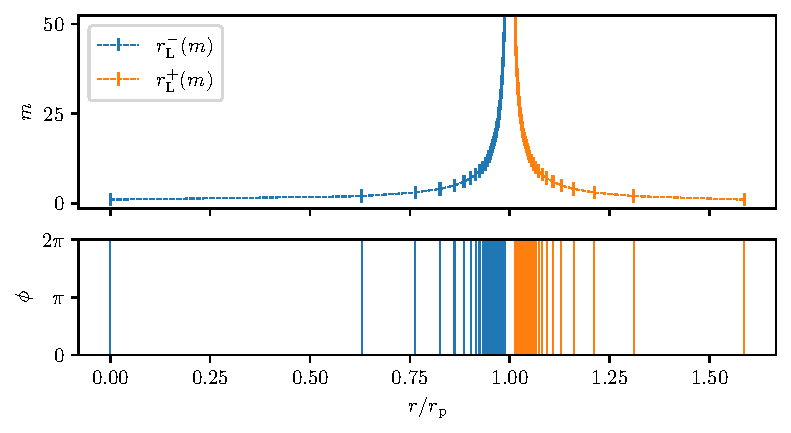
\includegraphics[width = 0.9\textwidth]{figures/lindblad_two_panel.pdf}
    \caption{\note{add caption}}
    \label{fig:lindblad}
\end{figure}

\subsection{The Planet Wake}

\note{add context: \citet{ogilvie2002}. We are not exactly following original derivation instead we want form of wake given in \citet{rafikov2002a}.}

Similarly to in section \ref{sec:linshu}, we can write linear wave quantities in a 2D gas disk as 
\begin{align}
    \delta a_m = A_m(r) \exp{i \Theta_m},
\end{align}
where the amplitude $A_m(r)$ varies slowly with radius and the phase
\begin{align}
    \Theta_m = \int^r k(r') \, dr' + m (\phi - \Omega_p t),
\end{align}
varies rapidly with radius. 
Again only the real component is physically relevant, and we have written $\omega = m \Omega_p$ as we are assuming the waves are generated by an embedded planet.
To investigate the shape of the spiral wake we will look for lines of constant phase that are defined by the condition $\frac{d\Theta_m}{dr} = 0$ and so 
\begin{align}
    \frac{d\phi}{dr} = - \frac{k}{m}. \label{eq:spiral_km}
\end{align}
This is the same as the relation used to find the pitch angle of the spiral shape in equation \ref{eq:pitchangle}.
Assuming Keplerian rotation such that $\kappa=\Omega=\Omega_{\rm K}$, we can find $k$ from the Lin-Shu Dispersion relation \ref{eq:lin_shu_disp}
\begin{align}
    k^2 &= \frac{m^2 \left( \Omega - \Omega_{\rm p} \right)^2 - \kappa^2}{c^2} \\
    &= \frac{m^2 \Omega_{\rm K}^2}{c^2} \frac{1}{r_{\rm p}^3} \left[ r^{3/2} - \left( r_{\rm L}^+ \right)^{3/2} \right] \left[ r^{3/2} - \left( r_{\rm L}^- \right)^{3/2} \right].
\end{align}
The tidal forcing of the planet results in density waves launched at the Lindblad resonances, with those launched at $r_{\rm L}^-$ and $r_{\rm L}^+$ propagating inwards and outwards through the disk respectively \citep{goldreich1978,goldreich1979}.
Figure \ref{fig:wakes_m3} shows the shape of the $m=3$ spiral waves generated at the $r_{\rm L}^\pm (m=3)$ Lindblad resonances as they propagate inwards and outwards through the disk.
The shape of these spirals is calculated as follows.
\begin{figure}[H]
    \centering
    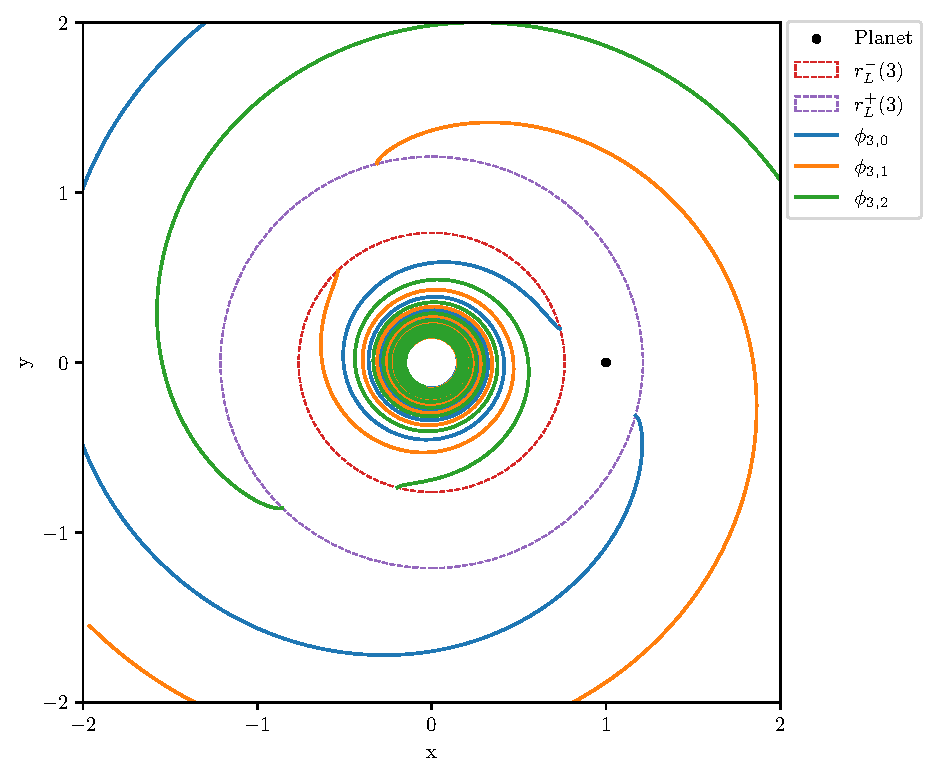
\includegraphics[width = 0.9\textwidth]{figures/wakes_m3.pdf}
    \caption{\note{add caption}}
    \label{fig:wakes_m3}
\end{figure}
Placing ourselves in the frame where the planet is stationary at $\phi = 0$, we can find the phase of the spiral waves simply by integrating equation \ref{eq:spiral_km} giving \citep{bae2018a}
\begin{align}
    \phi_m (r) = \phi_m(r_{\rm L}^\pm) - \int_{r_{\rm L}^\pm}^r \frac{k(r')}{m} \, dr', \label{eq:phase}
\end{align}
which consists of a constant offset $\phi_m(r_{\rm L}^\pm)$ which gives the azimuthal launching location, plus a term that varies with radius.
For the waves launched at the Lindblad resonances, the constant offset term can be found from the asymptotic behaviour of the Airy function \citep{ward1986}. 
For the $n$th arm of the $mth$ mode, where $n = 0, 1, ..., m-1$ the offset is given by 
\begin{align}
    \phi_{m,n}(r_{\rm L}^\pm) = - \sign (r_{\rm L}^\pm - r_{\rm p}) \frac{\pi}{4m} + 2 \pi\frac{n}{m}. \label{eq:spiral_offset}
\end{align}
Now considering the $n=0$ arm, we see from the above that it launches closest to $\phi=0$ and thus closest to the planet.
For large $m$, we find that the constant offset term $\phi_{m,0}(r)$ becomes independent of $m$.
In addition, we have that $r_{\rm L}^\pm \rightarrow r_{\rm p}$ as $m \rightarrow \infty$.
This results in the formation of a coherent, one-armed spiral wave centred on the planet, as \ref{eq:phase} and \ref{eq:spiral_offset} reduces to
\begin{align}
    \phi_{\infty,0}(r) = - \int_{r_{\rm p}}^ r \frac{\Omega(r') - \Omega_{\rm p}}{c(r')} \, dr'. \label{eq:planet_wake}
\end{align}
Because the $n=0$ waves launch almost in phase nearby the planet, as seen in figure \ref{fig:planet_wake}, the planet wake is always centred on the planet location. 
The above result was first found by \citet{ogilvie2002}, although they wrote it in a different form. 
They dubbed the resultant spiral wave the planet "wake" in analogy with the Kelvin wedge produced by a ship moving through water.
The form shown above was first found in \citet{rafikov2002a}.

\begin{figure}[H]
    \centering
    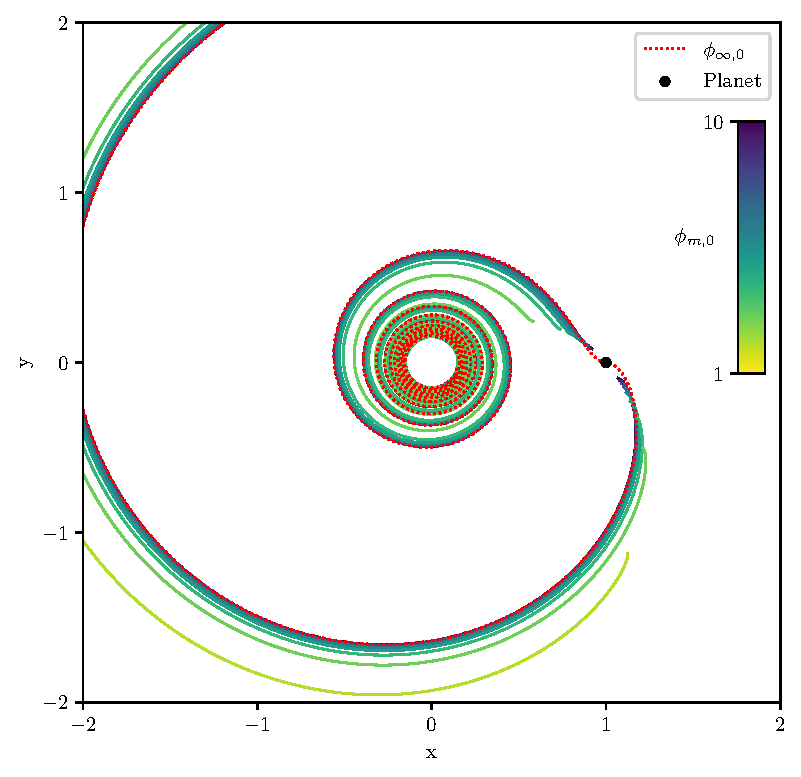
\includegraphics[width = 0.8\textwidth]{figures/planet_wake_shape.pdf}
    \caption{\note{add caption}}
    \label{fig:planet_wake}
\end{figure}

Ogilvie and Lubow also calculated the degree to which the constructive interference along $\phi_{\infty,0}$ fails.
To do this they calculated the relative error $\Delta_m$ in the phase for each $m$ caused by the approximation we have performed above.
Note that this is not the same quantity as we defined in \ref{eq:def_delta_m}.
Figure \note{add figure} shows $\Delta_m$ in both the outer and inner disk, for multiple values of $m$.
We see that in general, the approximation improves for larger $m$.
Additionally, the behaviour in the inner and outer disk is very different.
Ogilvie and Lubow found that $\Delta_m \sim \mathrm{constant}$ as $r \rightarrow \infty$, while $\Delta_m$ diverges as $r \rightarrow$ 0, and that for any fixed $r$ that $\Delta_m \rightarrow 0$ as $m \rightarrow \infty$.
Thus the accuracy of the one-armed wake shape \ref{eq:planet_wake} is in general better in the outer disk than the inner disk, and also depends on the importance of each mode.
If the wave is dominated by large $m$ then \ref{eq:planet_wake} holds everywhere except for very small disk radii, while always failing if dominated by $m=1$ or $2$ \citep{ogilvie2002}.
The dominating azimuthal mode for tidal forcing by a planet is $m_{\rm D} \approx 1/2 \left( H/r \right)_{\rm p}^{-1}$ \citep{goldreich1980}, and so for candidate planetary companions in observed disks $m_{\rm D} \gtrsim 5$ \fct. 
The coherent planet wake picture should therefore hold well except for at small disk radii.

\begin{figure}[H]
    \centering
    \begin{subfigure}[b]{0.49\textwidth}
        \centering
        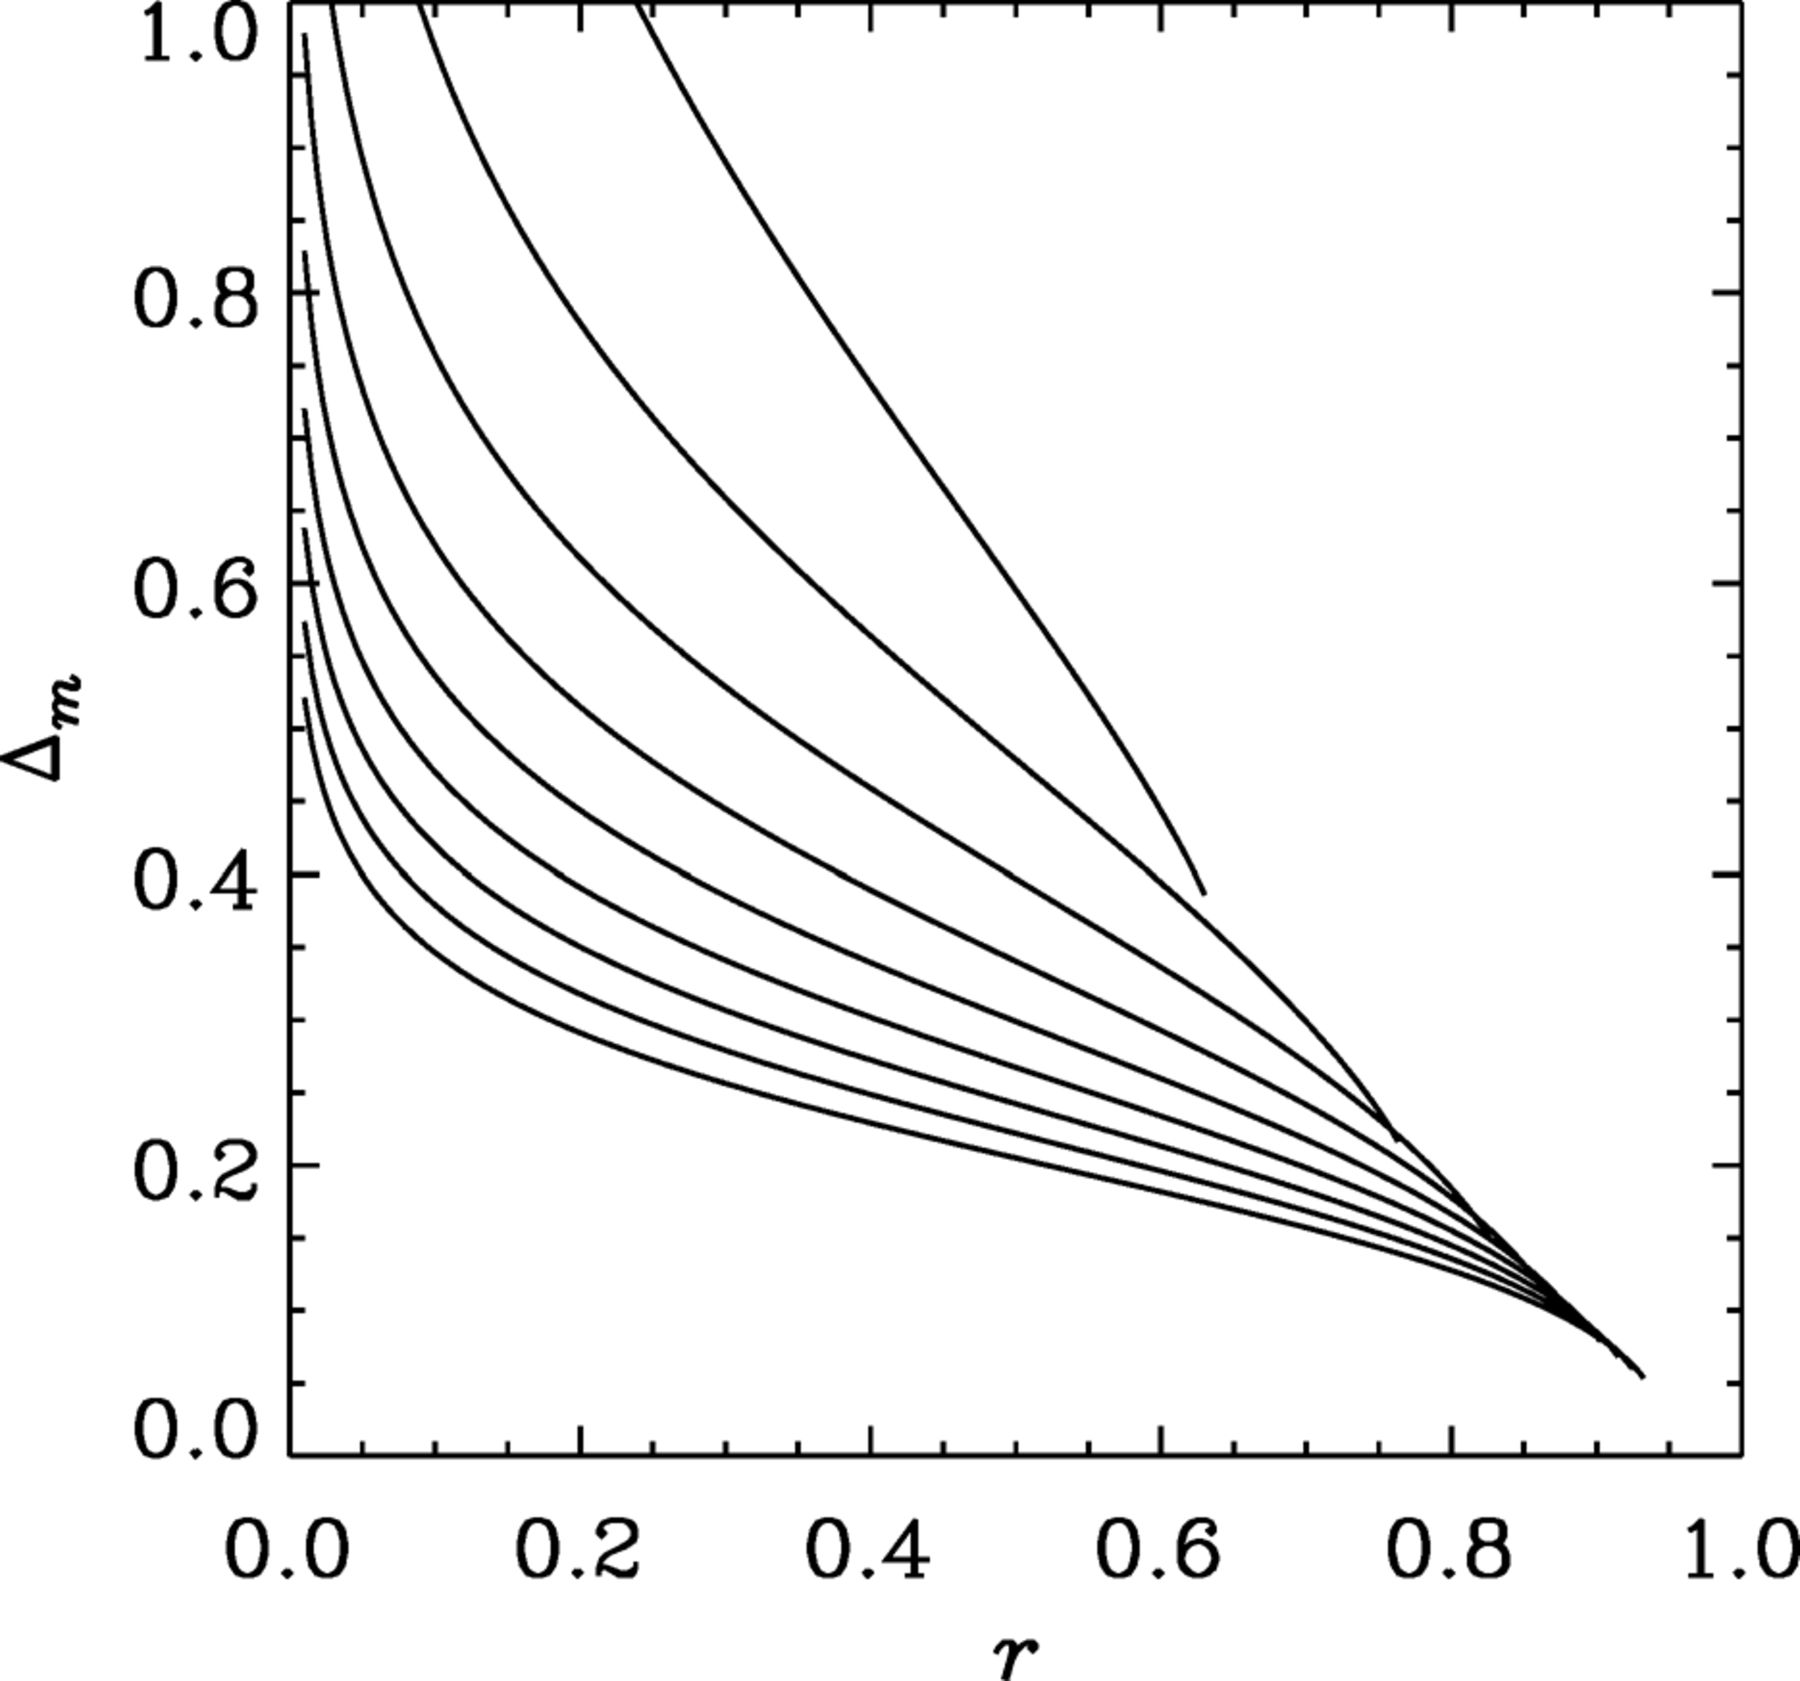
\includegraphics[width=\textwidth]{figures/Delta_m_inner.jpeg}
        %\caption{$y=x$}
        \label{fig:delta_m_inner}
    \end{subfigure}
    \hfill
    \begin{subfigure}[b]{0.49\textwidth}
        \centering
        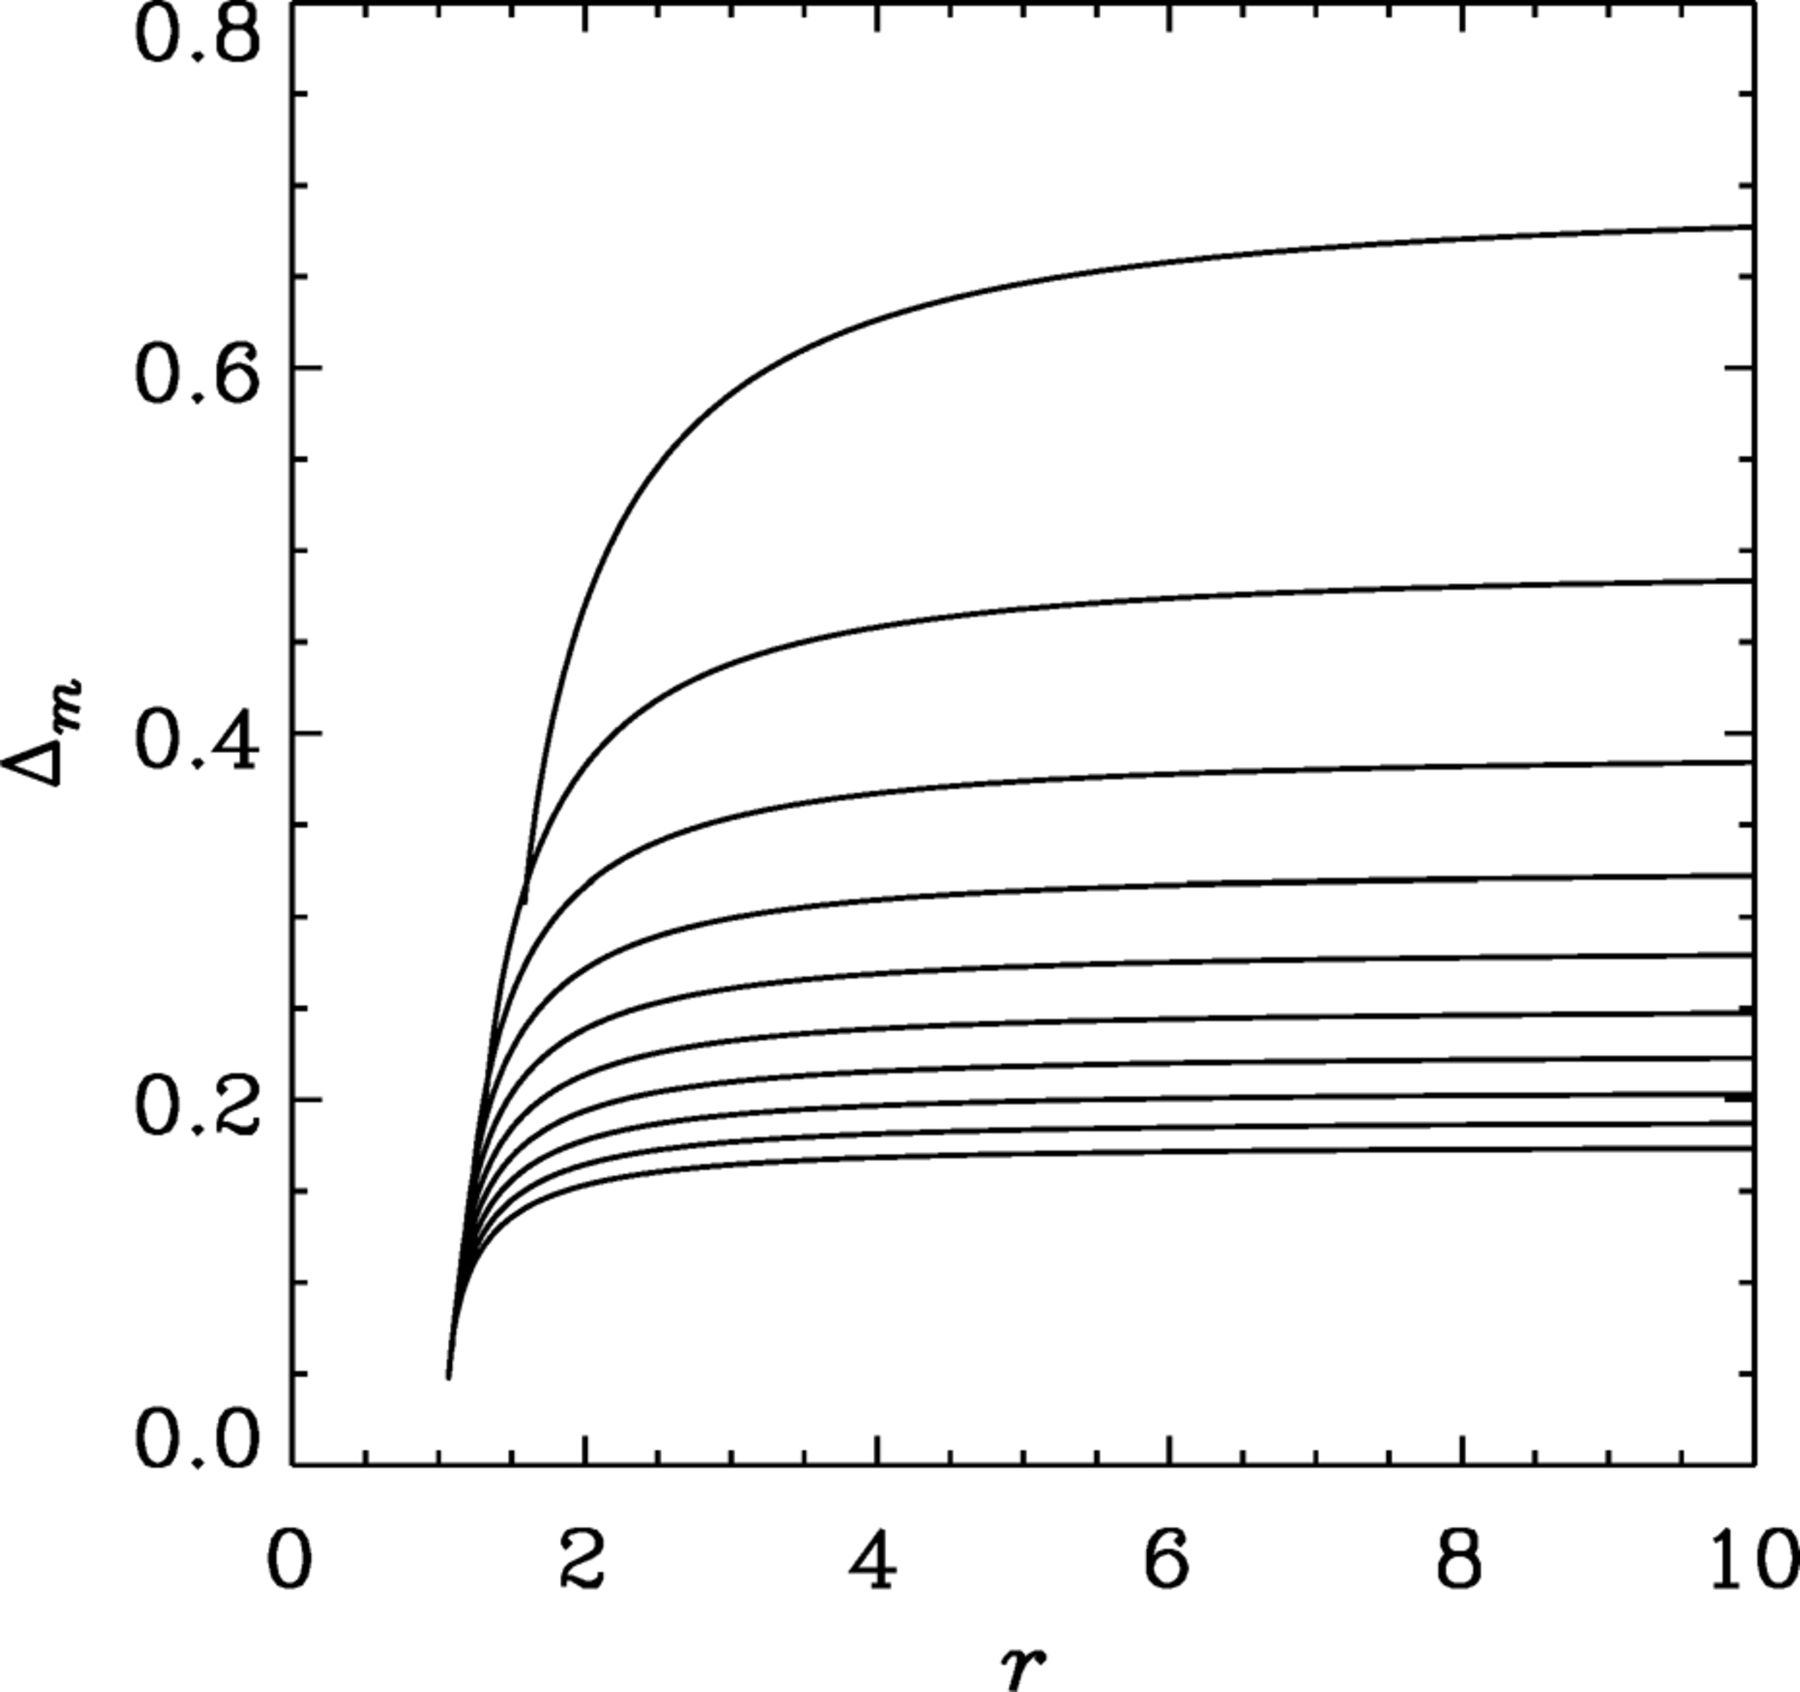
\includegraphics[width=\textwidth]{figures/Delta_m_outer.jpeg}
        %\caption{$y=3sinx$}
        \label{fig:delta_m_outer}
    \end{subfigure}
       \caption{\note{add caption}}
       \label{fig:delta_m}
\end{figure}

\subsection{Additional Spiral Arms}

In addition to constructive interference of the $n=0$ components causing the planet wake, it is possible for additional spiral arms to form.
These \textit{secondary} and \textit{tertiary} spiral arms (where the planet wake described in the previous section is the \textit{primary} arm) were first seen in numerical calculations \fct and were not very well understood in the context of linear density wave theory until quite recently \citep{bae2018a,miranda2019a}.
Unlike the primary, these spirals are not centred on the planet position, and are instead generated some distance away in the inner disk.

Figure \note{add figure} shows the phase of the $n=1$ and $n=2$ components in the inner disk.
We see that unlike for the $n=0$ case, the waves are not launched in the vicinity of the planet, or nearby each other.
However the overall behaviour of the constant offset launching term \ref{eq:spiral_offset} is the same for non-zero $n$, namely that it becomes smaller as $m$ increases and so the launching phases become closer for larger $m$.
Furthermore, the modes become more tightly wound as $m$ increases, with the second term of \ref{eq:phase} also losing its $m$ dependence for very large values.
These effects allow the larger $m$ modes launched closer to the planet to catch up to the low $m$ modes.
\citet{bae2018a} first performed this analysis and proposed that this catching up effect is responsible for the generation of secondary and tertiary spirals.
This also provides a natural explanation as to why the additional arms are not centred on the planet, as the interference only becomes coherent after the large $m$ modes have caught up in phase.
Bae and Zhu also found that this effect does not operate in the outer disk, as the difference in phase between small and large $m$ modes becomes constant instead of decreasing.

\begin{figure}[H]
    \centering
    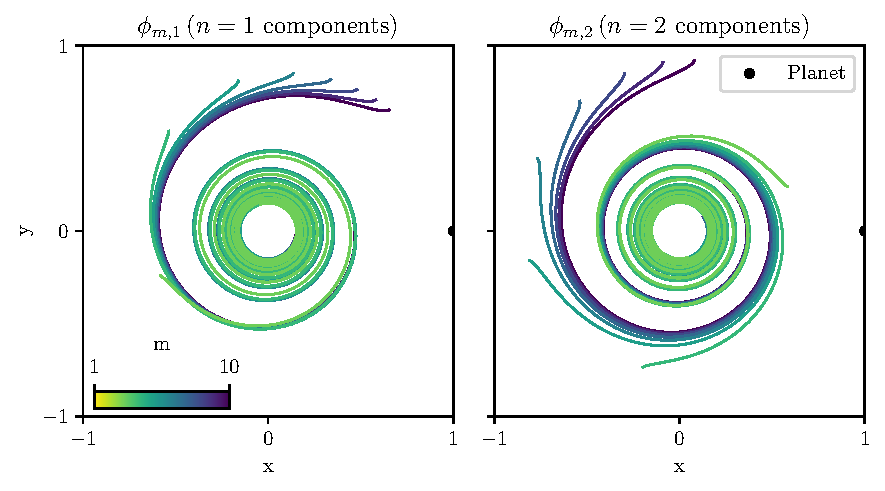
\includegraphics[width = 0.95\textwidth]{figures/inner_n_1_and_2.pdf}
    \caption{\note{add caption}}
    \label{fig:additional_arms}
\end{figure}

\citet{miranda2019a} built upon this work through numerical calculations and showed that the formation of additional arms in the inner disk is a robust prediction of the linear theory.
They did this by taking into account the global mode structure outside of the WKB approximation as used in \citet{bae2018a}, and calculated both the phase and amplitude of each mode.
They found that their results in general supported the picture of additional arms resultant from coincident phases, but that taking into account the amplitude information changes the level of correspondence and can be important, especially for the tertiary and higher order arms (those formed by $n>2$).

In this work we will be concerned primarily with the waves generated by the planet in the outer disk and so our models will not include any of the additional arms in the inner disk, only the primary planet wake.

\subsection{Linear}

\section{Non-Linear Wake Evolution}

\subsection{The Burger's Equation}

\subsection{Angular Momentum Flux}

\section{Gap Formation}